\section{Implementierung}

Die Implementierung der Interval-Events hat das gleiche Schema wie die
Implementierung der Events. Es handelt sich bei Intevall-Events um eine
spezielle Form von Event-Nodes die aus einem Start- und einem Stop-Event
bestehen.

Wie bei jedem Event-Node aus dem scala.events-Package durchläuft ein
Intervall-Event einen Lebenszyklus bestehend aus dem Setup des Event-Graphen,
der Registrierung von Reactions, dem Deploy, der Unregistrierung von Reactions
und dem Undeploy von Event-Nodes. Dieser Lebenszyklus ist auch in
Abb. \ref{event_node_lifecycle} zu sehen.

%\usepackage{graphics} is needed for \includegraphics
\begin{figure}[htp]
\begin{center}
  
\includegraphics[width=0.7\textwidth]{graphics/EventNode-Lifecycle}
  \caption[labelInTOC]{Lifecycle eines EventNodes}
  \label{event_node_lifecycle}
\end{center}
\end{figure}


Es gibt, wie in Abb. \ref{interval_events_structure} zwei Klassen von
Interval-Event-Nodes: BetweenEvents und ExecutionEvents. BetweenEvents sind vom
Auftreten des StartEvents bis zum Auftreten des ersten End-Events aktiv, wenn
eine Reaction registiert wurde\footnote{Dieses Verhalten ist näher im }

%\usepackage{graphics} is needed for \includegraphics
\begin{figure}[htp]
\begin{center}
  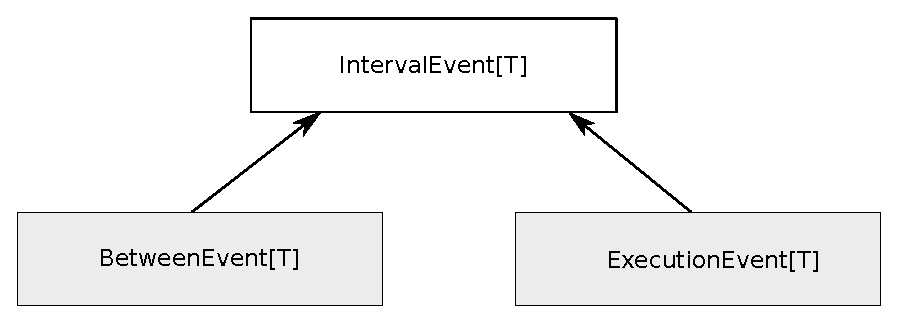
\includegraphics[width=0.5\textwidth]{graphics/interval_event_structure}
  \caption[labelInTOC]{Arten von Intervall-Events}
  \label{interval_events_structure}
\end{center}
\end{figure}

\subsection{Deploy-Verhalten von Intervall-Events}
Ein Intervall-Event wird genau dann deployed, wenn die Deploy-Methode des Start-
oder End-Events aufgerufen wird. 


\subsubsection{Einschränkungen der Implementierung}
In einem Event-Graph können nicht EventNodeRef oder EventNodeExists in einem
Pfad zusammen mit EventNodeExcept verwendet werden, da dies möglicherweise zu
nicht korrekten Ergebnissen führen würde.

Beim EventNodeExcept kann ein Except-Event empfangen werden, der das Entfernen
von Reactions auslöst. Die sorgt möglicherweise für Inkonsistenzen
bei Vorgängerknoten im Event-Graphen, wenn sich die Reaction des Except-Knotens
vor der Reaction eines anderen Knotens in der ReactionListe befindet.
Daher muss im Falle eines Except-Events immer ein Undeploy und ein Deploy
ausgeführt  werden, um die geänderten Reactions weiterzupropagieren.

Dies funktioniert allerdings nicht mehr länger mit EventNodeRef oder
EventNodeExists, dieses die Reihenfolge von Reactions verändern können.
